% project implementation and code descriptions (10-15 pages)
\chapter{Реализация на библиотека за създаване на текстов потребителски}
\hfill

\section{Структура на проекта}

        Всички части на библиотеката се намират в пакета tui, който от своя 
        страна е разделен на подпакети:
        \begin{itemize}
                \item стилизация - styles
                \item елементи - components
                \item събития - events
        \end{itemize}

        \begin{figure}[H]
                \centering
                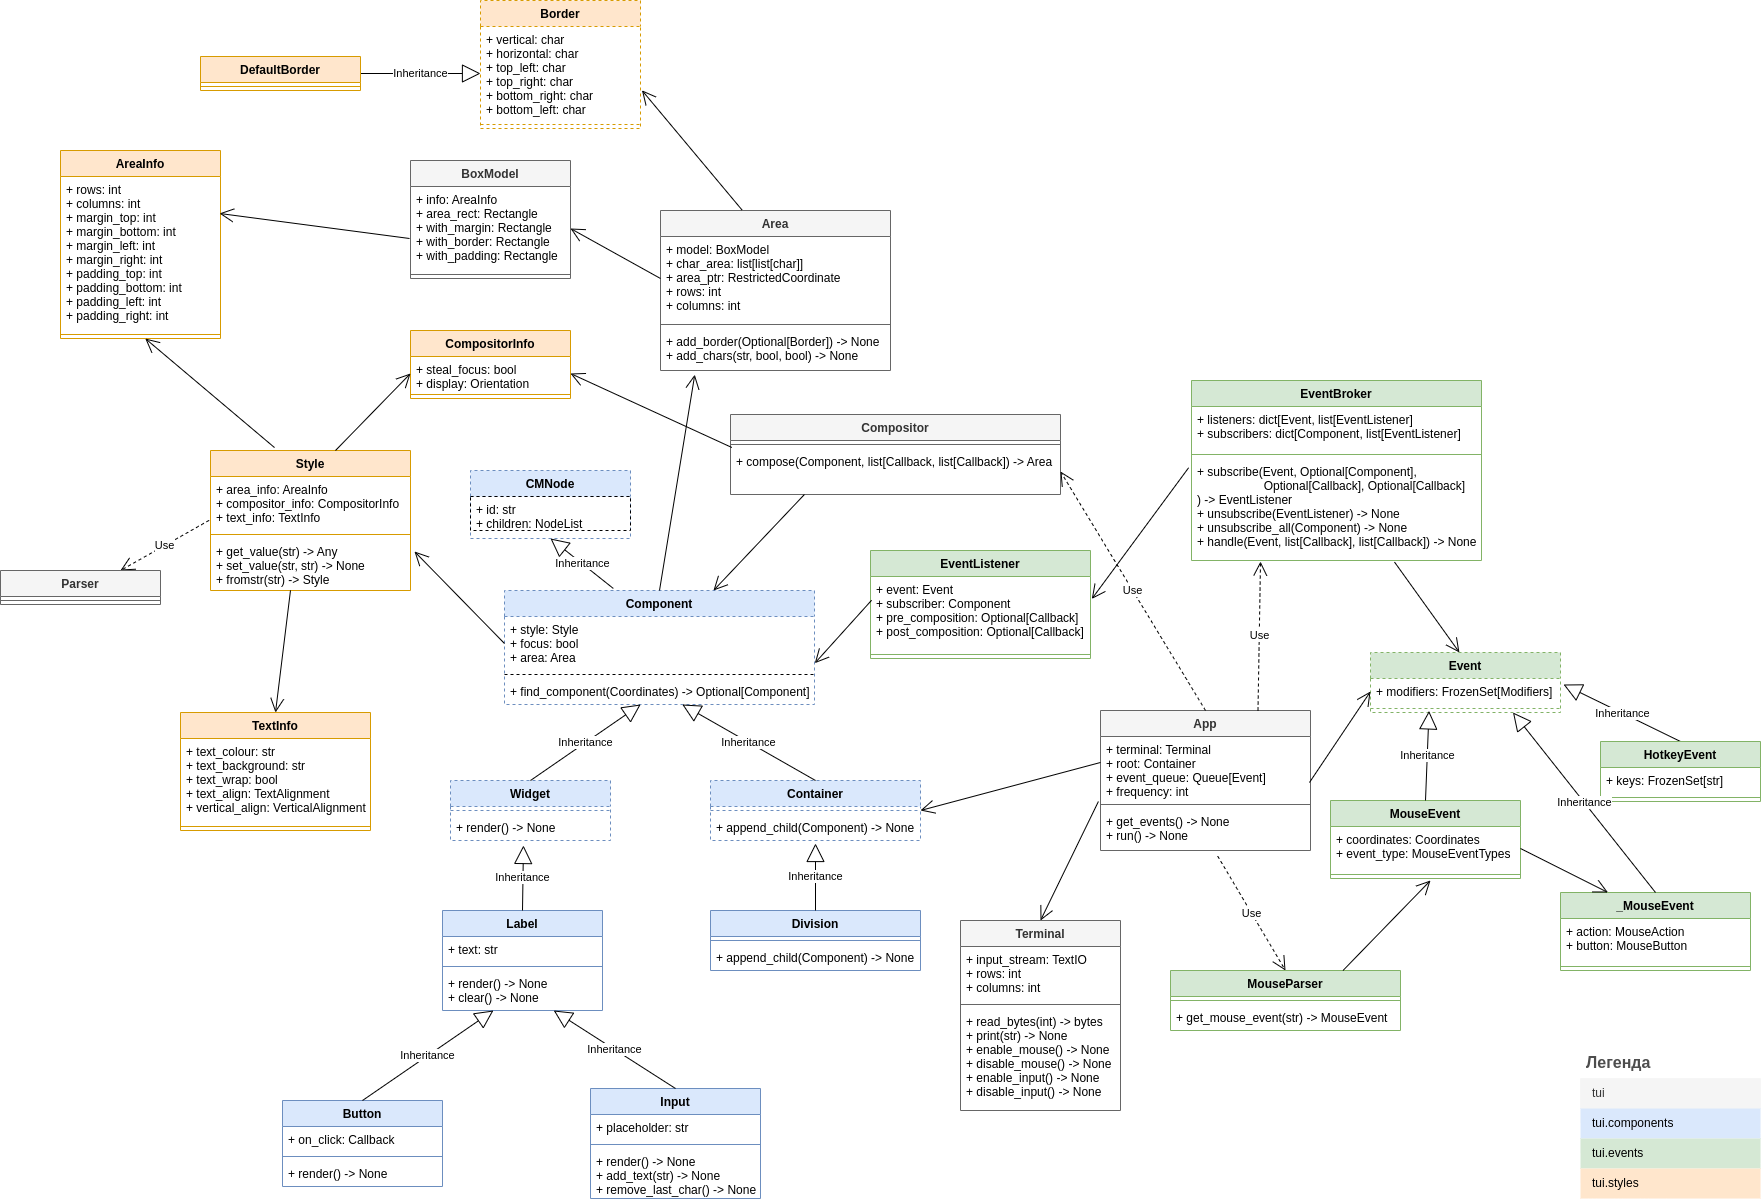
\includegraphics[
                        angle=0,
                        origin=center,
                        width=\linewidth
                ]{images/uml-tui.drawio.png}
                \caption{UML диаграма на архитектурата на библиотеката}
                \label{fig:architecture-uml}
        \end{figure}
        \vspace{10mm}

\section{Файлове с общо предназначение}

        Фаловете \textbf{\_coordinates.py} и \textbf{\_parser.py} са с общо 
        предназначение.
        \newline

        Във файла \textbf{\_parser.py} са дефинирани регулярни изрази (regex),
        които се използват в целия проект.

        Файлът \textbf{\_coordinates.py} предоставя абстракция за точка в
        декартова координатна система, правоъгълник и точка, която не може да
        излезе извън границите на правоъгълник.

\section{Йерархия на компоненти}

        Всяко приложение има главен (root) компонент, който обикновено заема 
        цялата резолюция на терминала. Към този компонент могат да се добавят
        деца - други компоненти, които описват как изглежда главният компонент
        - родителят им. Този процес може да се повтори за всички компоненти,
        които могат да имат деца, като по този начин се образува дървовидна
        структура наподобяваща документен обектен модел (ДОМ).

        \begin{figure}[H]
                \centering
                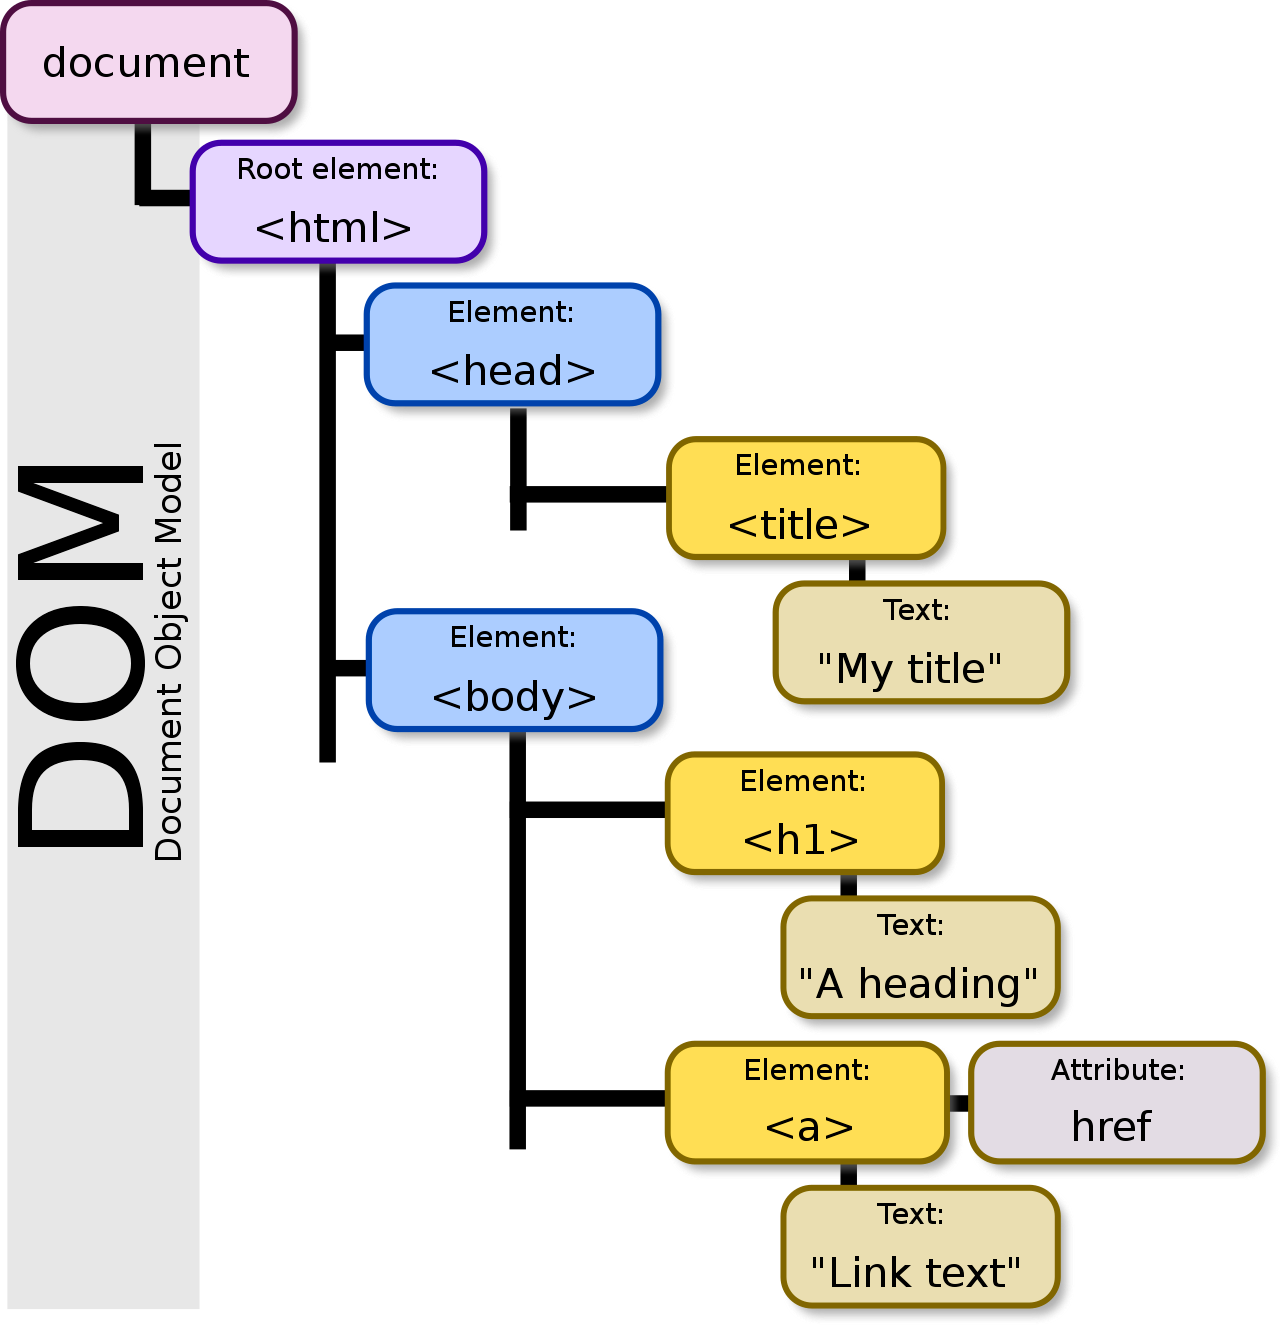
\includegraphics[
                        angle=0,
                        origin=center,
                        width=90mm
                ]{images/dom-tree.png}
                \caption{Пример за ДОМ дърво}
                \label{fig:DOM-tree}
        \end{figure}
        \vspace{10mm}

        Компонентното дърво е имплементирано посредством класа 
        \textbf{NodeList}. Компонентите се записват в:
        \begin{itemize}
                \item масив - запазва реда на компонентите
                \item хеш таблица - откриването на компонент според
                        идентификатора му отнема константо време.
        \end{itemize}

        \hspace{1mm}
        % NodeList code
        \begin{lstlisting}[style=py]
class NodeList(Sequence):
    """Responsible for providing a structure for accessing an ordered component list"""

    def __init__(self) -> None:
        self._nodes_list: list[Component] = []  # preserve order
        # components with no id aren't in the dict
        self._nodes_dict: dict[str, Component] = {}  # fast search by index

    def __len__(self) -> int:
        return len(self._nodes_list)

    def __getitem__(self, index: int | slice) -> Component | list[Component]:
        return self._nodes_list[index]

    def __setitem__(self, index: int, new_component: Component) -> None:
        prev_component = self._nodes_list[index]
        self._nodes_list[index] = new_component

        if prev_component.id is not None:
            self._nodes_dict.pop(prev_component.id)
        if new_component.id is not None:
            self._nodes_dict[new_component.id] = new_component

    def __contains__(self, component: Component) -> bool:
        return component in self._nodes_list

    def get_by_id(self, identifier: str) -> Optional[Component]:
        """Get component (search by id)"""
        return self._nodes_dict.get(identifier)

    def append(self, component: Component) -> None:
        """Add component at the end of the list"""
        if component in self._nodes_list:
            raise ValueError("Component already exists")

        if component.id in self._nodes_dict:
            raise KeyError("Id already exists")

        self._nodes_list.append(component)

        if component.id is not None:
            self._nodes_dict[component.id] = component

    def pop(self, index: int) -> Component
        """Remove component (search by id)"""
        component = self._nodes_list.pop(index)

        if component.id is not None:
            self._nodes_dict.pop(component.id)

        return component

    def remove(self, component: Component) -> None:
        """Remove component"""
        self._nodes_list.remove(component)
        if component.id is not None:
            self._nodes_dict.pop(component.id)
        \end{lstlisting}

\section{Вътрешно представяне на компонент}
        Както се забелязва \figref{fig:architecture-uml}, компонентите зависят
        от класа \textbf{Area}. Това е задължителна част от всеки компонент. В 
        основата си, класът представлява двуизмерна матрица от символи, която 
        определя как трябва да изглежда даден компонент сам по себе си - преди 
        да бъде композиран. 

        \hspace{5mm}
        \begin{lstlisting}[style=py]
class Area:
    """
    Responsible for rendering how a component should look.
    This includes the box model and any dynamic changes that may happen within it
    """
    def __init__(self, area_info: AreaInfo, border: Optional[Border] = None) -> None:
        self.model = BoxModel(info=area_info)
        # char_area is where every change is reflected
        # rows x columns
        self.char_area: list[list[str]] = [
                [' ' for _ in range(self.columns)]
                for _ in range(self.rows)
            ]

        # the area pointer is used for easier navigating and writing to
        # char_area as it automatically keeps track of a lot of variables
        self.area_ptr = RestrictedCoordinates(
                    _row=0,
                    _column=0,
                    _restriction=self.model.with_padding,
                    relative=True
                )

        self.add_border(border)

    def __str__(self):
        return "\n".join(["".join(list(row)) for row in self.char_area])

    def add_border(self, border: Optional[Border]) -> None:
        """Apply border to the area. This will shrink the space the component
        can use depending on the border's size"""

        ... # code omitted

    def add_chars(
            self,
            string: str,  # string to be added to the area
            column_preserve: bool = False,  # should new line start at the current area pointer column
            ptr_preserve: bool = True  # reset area pointer to initial position
    ) -> None:
        """Write to char_area starting from area_ptr coordinates.
        Any '\n' in the string translate to a row increment.
        Default behaviour doesn't mutate the area pointer."""

        # remember initial coordinates (for column preserve and to roll-back the area pointer)
        initital_coords = Coordinates(_row=self.area_ptr.row, _column=self.area_ptr.column)

        # check if string can fit
        if not self._verify_str(
                string=string,
                column_preserve=column_preserve
        ):
            raise IndexError("String is too large")

        for count, char in enumerate(string):
            if char == '\n':
                # if area_ptr is on the last row and the last char is a newline
                # area_ptr restriction would activate, hence the latter check
                if count >= len(string) - 1:
                    break

                self.area_ptr.row += 1
                if column_preserve:
                    self.area_ptr.column = initital_coords.column
                else:
                    self.area_ptr.column = (
                            self.area_ptr.restriction.top_left.column
                        )

                continue

            self.char_area[self.area_ptr.row][self.area_ptr.column] = char

            # Required check to prevent a RestrictedCoordinates exception
            if (self.area_ptr.column < self.area_ptr.restriction.bottom_right
                    .column):
                self.area_ptr.column += 1

        if ptr_preserve:
            self.area_ptr.row = initital_coords.row
            self.area_ptr.column = initital_coords.column
        else:
            # column is incremented one last time after adding the last char
            # this can force area_ptr to go out of bounds hence returning the pointer one back
            self.area_ptr.column -= 1

    def _verify_str(self, string: str, column_preserve: bool) -> bool:
        """Verify that string can fit in char_area - used in add_chars.
        It mimics the behaviour of add_char to make sure the string never goes out of bounds."""

        ... # code omitted


    ... # methods omitted
        \end{lstlisting}


\section{Видове компоненти}
        Компонентите могат да се разделят на две категории, в зависимост от
        поведението си:

        \begin{itemize}
                \item \textbf{Container} - Отговаря единствено за собствените 
                        си деца. Управлява реда, в които ще се композират и
                        позициите, в които ще застанат едни спрямо други.
                        Примерна имплементация на контейнер е \textbf{Division}
                        (разделение)
                        \vspace{5mm}
                        \begin{lstlisting}[style=py]
class Container(Component):
    """
    Abstract component that's responsible for containing and organizing other components.
    `@property def children(self)` should be implemented in child classes
    """

    def __init__(
            self,
            *children: Component,  # Child components
            style: str | Style = Style(),  # Style properties for the component
            identifier: Optional[str] = None,  # Unique identifier
    ) -> None:
        super().__init__(identifier=identifier, style=style)

        for child in children:
            # Components that inherit Container could pass *children to
            # super().__init__() which is seen as an empty tuple here
            if isinstance(child, tuple):
                continue

            self.append_child(child)

    def append_child(self, component: Component):
        """Add a child at the end of the component list of the container.
        You can manipulate this by adding other components for positioning or composition"""
        self.children.append(component)
                        \end{lstlisting}
                \vspace{5mm}
                \item \textbf{Widget} - Абстрактен компонент, който не може да
                        има дъщерни компоненти. Може да променя поведението на 
                        повечето събития и се съсредоточава върху изъплняването
                        на конкретна функционалност. Примери за уиджети са 
                        класовете \textbf{Label} (надпис) и \textbf{Button}
                        (бутон).

                        \vspace{11mm}
                        \begin{lstlisting}[style=py]
class Widget(Component):
    """An abstract component that can't hold other components and can override event behaviour."""
    def __init__(
            self,
            style: str | Style = Style(),  # Style properties for the component
            identifier: Optional[str] = None,  # Unique identifier
    ) -> None:
        super().__init__(identifier=identifier, style=style)

    @abstractmethod
    def _render_to_area(self) -> None:
        """Render the component's content to its area"""

    @property
    def children(self) -> list:
        """Widgets can't have child components. 
        Return an empty list for compatibility"""
        return []
                        \end{lstlisting}
        \end{itemize}

        Благодарение на разграничението на компоненти, всеки изпълнява само 
        една роля (SRP). Това улеснява имплементирането на нови компоненти, 
        като композиция от вече съществуващи компоненти.

\section{Композитор}

        Композиторът е съставна част от приложението. Той се грижи за 
        сглобяването на крайния му изглед. Процесът се изпълнява 
        във всеки кадър при условие, че има промяна на изгледа. Алгоритъмът се
        основава на ОД (обхождане в дълбочина).

        Методът \textbf{compose} се извиква рекурсивно с всички деца на главния
        (root) компонент, докато не се стигне до най-крайното дете - дете, 
        което няма деца. Неговият родител получава вътрешното му представяне и
        го подрежда според стила си. Текущият проект поддържа два вида 
        ориентация на контейнери:
        \begin{itemize}
                \item \textbf{inline} - децата на контейнера се подреждат на
                        същия ред
                \item \textbf{block} - децата на контейнера се подреждат в 
                        същата колона
        \end{itemize}

        \vspace{5mm}
        \begin{lstlisting}[style=py]
class Compositor:
    """Responsible for compositing components into a single area"""

    @staticmethod
    def compose(
            root: Component,  # the component which's area is being composed
            pre_composit: list[Callback],
            post_composit: list[Callback]
    ) -> Area:
        """Compose a component with its children components recursively. Run
        pre-compose and post-compose hooks"""
        for callback in pre_composit:
            callback()

        # set root rect mapping to itself
        root._rect_mapping = root.area.model.area_rect
        new_area = Compositor._compose(root=root)

        for callback in post_composit:
            callback()

        return new_area

    @staticmethod
    def _compose(root: Component) -> Area:
        """Compose a component with its children components recursively

        root: the component's area that's being composed
        next_component: rectangular area which the next component should occupy
        """

        new_area = copy.deepcopy(root.area)

        # the rectangle the previous child was in
        prev_rect: Optional[Rectangle] = None

        for child in root.children:
            try:
                prev_rect = Compositor._get_next_rectangle(
                        parent=root,
                        prev_rect=prev_rect,
                        component=child
                    )
                child._row_mapper = prev_rect
            except CoordinateError as exc:
                raise InsufficientAreaError(
                        "Component area isn't large enough"
                    ) from exc

            # recursion ends when there are no more children
            child_area = Compositor._compose(child)
            new_area.area_ptr.row = (
                prev_rect.top_left.row
                + new_area.model.with_padding.top_left.row
            )
            new_area.area_ptr.column = (
                prev_rect.top_left.column
                + new_area.model.with_padding.top_left.column
            )

            # draw child component
            try:
                new_area.add_chars(str(child_area), column_preserve=True)
            except IndexError as exc:
                raise InsufficientAreaError(
                        "Component area isn't large enough"
                    ) from exc

        return new_area

    @staticmethod
    def _get_next_rectangle(
            parent: Component,  # the parent component this one will reside in
            component: Component,  # the component calculations are done for
            prev_rect: Optional[Rectangle] = None
    ) -> Rectangle:
        """Helper function that decides where components are placed when
        compositing"""
        if parent.style.compositor_info.display == Orientation.INLINE:
            return Compositor.__get_next_rectangle_inline(
                    parent=parent,
                    component=component,
                    prev_rect=prev_rect
                )

        return Compositor.__get_next_rectangle_block(
                parent=parent,
                component=component,
                prev_rect=prev_rect
            )

    @staticmethod
    def __get_next_rectangle_inline(
            parent: Component,  # the parent component this one will reside in
            component: Component,  # the component calculations are done for
            # rectangle for the previous component
            prev_rect: Optional[Rectangle] = None
    ) -> Rectangle:
        """Helper function for inline compositing. Returns the area the next
        component should be placed in

        Default prev_rectangle is a rectangle outside of the parent's area
        that's derived to place the component in the top left of the parent
        component's area:
            top_left:  row = 0 && column <= -1
            bottom_right:  row >= 0 && column = -1
        """
        if prev_rect is None:
            prev_rect = Rectangle(
                    top_left=Coordinates(_row=0, _column=-1),
                    bottom_right=Coordinates(_row=0, _column=-1)
                )

        return Rectangle(
                top_left=Coordinates(
                        _row=prev_rect.top_left.row,
                        _column=prev_rect.bottom_right.column + 1
                    ),
                bottom_right=Coordinates(
                        _row=parent.area.rows - 1,
                        _column=prev_rect.bottom_right.column +
                        component.area.columns
                    )
            )

    @staticmethod
    def __get_next_rectangle_block(
            parent: Component,  # the parent component this one will reside in
            component: Component,  # the component calculations are done for
            # rectangle for the previous component
            prev_rect: Optional[Rectangle] = None
    ) -> Rectangle:
        """Helper function for block compositing. Returns the area the next
        component should be placed in

        Default prev_rectangle is a rectangle outside of the parent's area
        that's derived to place the component in the top left of the parent
        component's area:
            top_left:  row = -1 && column <= 0
            bottom_right:  row >= -1 && column = 0
        """
        if prev_rect is None:
            prev_rect = Rectangle(
                    top_left=Coordinates(_row=-1, _column=0),
                    bottom_right=Coordinates(_row=-1, _column=0)
                )

        return Rectangle(
                top_left=Coordinates(
                        _row=prev_rect.bottom_right.row + 1,
                        _column=prev_rect.top_left.column
                    ),
                bottom_right=Coordinates(
                        _row=prev_rect.bottom_right.row + component.area.rows,
                        _column=parent.area.columns - 1
                    )
            )

        \end{lstlisting}

\section{Визуализация на приложение}

        Тъй като приложението е предвидено да се използва в терминал, кадрите в
        секунда, които могат да се постигнат, са ограничени от бодовете на 
        терминала. Писането в стандартния изход (stdout) трябва да използва 
        минимално системни извиквания, както и да се пишат минимален брой 
        байтове. За целта се използва техника подобна на двойно буфериране.
        \figref{fig:double-buffering}.
        
        \begin{figure}[H]
                \centering
                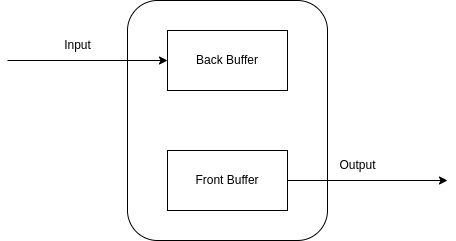
\includegraphics[
                        angle=0,
                        origin=center,
                        width=90mm
                ]{images/double-buffering.drawio.png}
                \caption{Принцип на работа на двойно буфериране}
                \label{fig:double-buffering}
        \end{figure}

        Използвайки аналогията с двойно буфериране 
        \figref{fig:double-buffering} - задният буфер запазва предишното 
        състояние - \textbf{Area}, на терминала. Сравнява се с текущото 
        състояние, като на предния буфер се записва низ, който описва промените
        с минимален брой байтове - използват се ANSI кодове за манипулиране на 
        позицията на курсора.

        \vspace{5mm}
        \begin{lstlisting}[style=py]
class Terminal:
    """Responsible for providing an interface to the terminal the program is being ran in"""

    def __init__(self, input_stream: TextIO = stdin) -> None:
        ... # code omitted
        self._prev_state: Optional[Are] = None
        ... # code omitted

    def print(self, area: Area) -> None:
        """Print a string to the terminal. Overwrites content in the terminal
        for higher response time and no stuttering."""
        # handle first print
        if self._prev_state is None:
            print(str(area), end="", flush=True)
            self._prev_state = area

            return

        print(self._mutate_on_diff(self._prev_state, area),
              end="",
              flush=True)
        self._prev_state = area

    def _mutate_on_diff(self, area1: Area, area2: Area) -> str:
        """Find the difference between 2 strings and return a string which
        describes how the first one should change to become the second. Assume
        that both strings have the same dimensions. Expected strings are
        unnecessarily bloated for this sole reason (a lot of whitespaces can be
        followed by '\n') """
        mutate_str = ""

        # are the char differences consecutive
        streak = False

        for line_count, line1 in enumerate(area1.char_area):
            for char_count, char1 in enumerate(line1):
                char2 = area2.char_area[line_count][char_count]
                if char1 != char2:
                    if streak is False:
                        # move cursor
                        mutate_str += self._move_cursor(row=line_count,
                                                        column=char_count)
                        streak = True

                    mutate_str += char2
                else:
                    streak = False

        return mutate_str

    def _move_cursor(self, row: int, column: int) -> str:
        """Return an ANSI code which moves the string to the specified
        coordinates."""
        return f"\x1b[{row};{column}f"

    ... # methods omitted
        \end{lstlisting}


\section{Персонализиране на компоненти}

        Всеки компонент може да бъде стилизиран посредством класа 
        \textbf{Style}. Това най-често се случва, като се подаде символен низ,
        на метода \textbf{fromstr}. Символният низ се обработва с регулярен
        израз (regex) и превръща в композиция от следните подстилове:

        \begin{itemize}
                \item \textbf{AreaInfo}
                \item \textbf{CompositorInfo}
                \item \textbf{TextInfo}
        \end{itemize}

        Валиден символен низ следва следния формат: 'property=value, ... '

\section{Издаване и обработка на събития}
        
        Текушият проект разпознава натискането на единични клавиши, комбинация
        от клавиши, когато e поддържана емулация на VT100 терминал, и събития
        от мишка в xterm терминални емулатори.

        Тези събития се прочитат от стандартния вход (stdin) и обработват с
        помощта на речници и регулярни изрази. Това се случва в отделна нишка
        по следния начин:

        \vspace{10mm}
        \begin{lstlisting}[style=py]
class App:
    """Contains everything necessary for running the application."""

    ... # methods omitted

    def get_events(self) -> None:
        """Continuously fetch events and put them in the event queue."""
        from tui.events._mouse_parser import MouseParser
        from tui.events.key_event import HotkeyEvent
        from tui.events.keys import ANSI_SEQUENCES_KEYS

        while True:
            # read from stdin
            control_code = self.__terminal.read_bytes(_bytes=16).decode()
            # check if it's a control sequence or a simple key press
            if len(control_code) == 1:
                self.event_queue.put(HotkeyEvent(control_code))
                continue

            # check if it's a mouse control code and add to the event queue
            try:
                self.event_queue.put(HotkeyEvent(ANSI_SEQUENCES_KEYS[control_code]))
            except KeyError:
                self.event_queue.put(MouseParser.get_mouse_event(control_code))

    ... # methods omitted

        \end{lstlisting}
        

\section{Абониране за събития}

        Принципът на работа със събития е много сходен до модела издател-абонат
        (pub-sub):

        \begin{figure}[H]
                \centering
                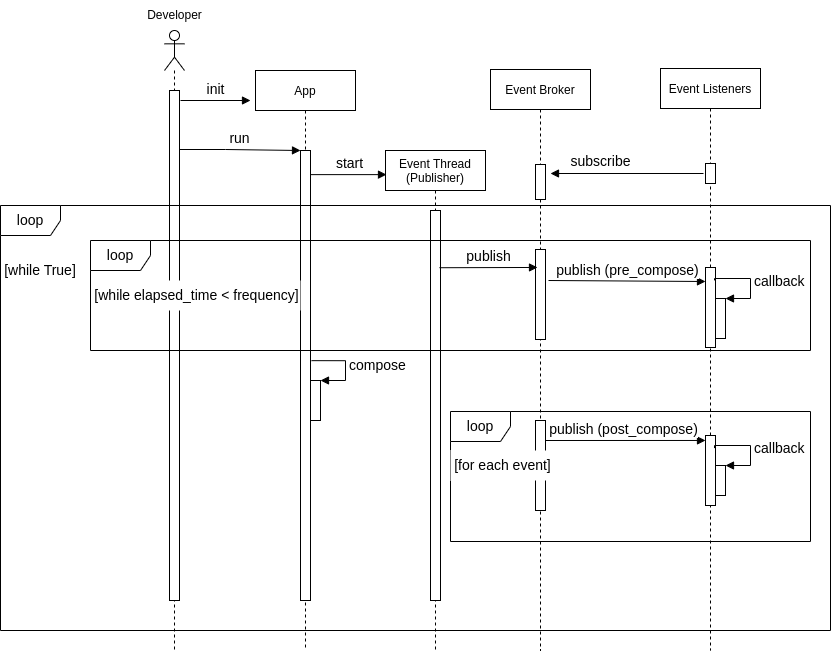
\includegraphics[
                        angle=0,
                        origin=center,
                        width=\linewidth
                ]{images/event-sequence-diagram.drawio.png}
                \caption{Sequence Диаграма на модела на работа със събития}
                \label{fig:event-sequence-diagram}
        \end{figure}

        Всеки компонент може да бъде абонат, но за да слуша за събития, 
        компонентът трябва да има фокус. Единствено глобалните абонати - 
        абонати без посочен компонент, не се нуждаят от фокус. Фокусът може да 
        се придобие посредством следния глобален абонат:

        \vspace{5mm}
        \begin{lstlisting}[style=py]
class App:
    """Contains everything necessary for running the application."""
    def __init__(
            self,
            fps: int = 60,  # frames per second
            # static row and col amount (in case terminal fails)
            rows: Optional[int] = None,
            columns: Optional[int] = None,
    ) -> None:

        ... # code omitted

        def set_focus(event: MouseEvent) -> None:
            """Set focus to a component, once it's clicked"""
            focus_component = self.root.find_component(event.coordinates)
            if focus_component is None or focus_component == set_focus.prev_component:
                return

            set_focus.prev_component._focus = False
            focus_component._focus = True
            set_focus.prev_component = focus_component

        set_focus.prev_component = None
        EventBroker.subscribe(
                event=MouseEventTypes.MOUSE_LEFT_CLICK,
                subscriber=None,
                pre_composition=set_focus
        )

        ... # methods omitted

        \end{lstlisting}

        Структурата на \textbf{EventListener} (абонат) съдържа следните полета:

        \begin{itemize}
                \item \textbf{event} - събитието, за което абонатът ще бъде 
                        известяван
                \item \textbf{subscriber} - компонентът, който трябва да има 
                        фокус, преди да започне да бъде известяван за събития.
                        Глобалните абонати са имплементирани посредством
                        компонент \textbf{subscriber}, който има идентификатор
                        равен на -1.
                \item \textbf{pre\_composition} - Функция, която ще се извика 
                        при известяване от събитие. Функцията се извиква преди
                        композирането на компоненти.
                \item \textbf{post\_composition} - Функция, която ще се извика
                        при известяване от събитие, след като е извършена 
                        композицията. Не може да се очаква синхроност с
                        pre\_composition, защото при възникването на
                        еднакви събития в период по-малък от един кадър, 
                        pre\_composition ще се извика два пъти преди
                        post\_composition да се извика два пъти. За
                        обработването на повечето събития се предпочита 
                        pre\_composition. Глобалният абонат за показване на 
                        курсора на мишка използва именно post\_compostion.
        \end{itemize}

        \textbf{EventBroker} класът има ролята на посредник между нишката, 
        която обработва събития, и абонатите, които очакват да бъдат известени.
        Той е отговорен за управлението на абонати, като предоставя методи за 
        абониране и отписване. При подаване на събитие към метода 
        \textbf{handle} определя кои \textbf{pre\_composition} и 
        \textbf{post\_composition} функции трябва да бъдат извикани.

        \begin{lstlisting}[style=py]
class EventBroker:
    """Responsible for managing event subscription and event callbacks"""

    # a 'subscriber' with id ==  -1 is used to signify a global event
    __global_component = Division(identifier='-1')

    listeners: dict[Event, list[EventListener]] = {}
    subscribers: dict[Component, list[EventListener]] = {}

    ... # methods omitted

    @staticmethod
    def handle(
            event: Event,
            pre_composit_hook: list[Callback],
            post_composit_hook: list[Callback]
    ) -> None:
        """Find the corresponding listeners for an event and prepare their
        callbacks. The callbacks are appended to the pre/post composite hooks.
        """

        def handle_listener(listener: EventListener, event: Event) -> None:
            if listener.pre_composition is not None:
                pre_composit_hook.append(
                        lambda: listener.pre_composition(event)
                    )
            if listener.post_composition is not None:
                post_composit_hook.append(
                        lambda: listener.post_composition(event)
                    )

        # Convert MouseEvent to _MouseEvent, since that is what listeners are
        # subscribed to
        if isinstance(event, MouseEvent):
            _event = event.event.value
        else:
            _event = event

        try:
            for listener in EventBroker.listeners[_event]:
                handle_listener(listener, event)

        except KeyError:
            # Do nothing if event isn't listened to
            return

        # handle listeners to all keys
        try:
            if not isinstance(event, HotkeyEvent):
                return
            for listener in EventBroker.listeners[HotkeyEvent(Keys.Any)]:
                handle_listener(listener, event)
        except KeyError:
            # Do nothing if event isn't listened to
            return
        \end{lstlisting}

        В основния цикъл на текущия проект се заемат събития от опашка, в която
        пише нишката, която чете и обработва събития. \textbf{EventBroker}
        дава достъп до всички абонати на текущото събитие.
        \textbf{pre\_composition} функциите се извършват между всеки кадър. За
        всеки кадър се композира \textbf{root} компонента, който след това се 
        принтира по максимално ефективен начин.
        % TODO: update code

        \begin{lstlisting}[style=py]
            
class App:
    """Contains everything necessary for running the application."""

    ... # methods omitted

    def run(self) -> None:
        """Start and constantly update the app."""
        input_thread = threading.Thread(
                target=self.get_events,
                args=(),
                daemon=True
            )

        input_thread.start()

        try:
            pre_composit_hook = []
            post_composit_hook = []
            timer_start = perf_counter()
            while True:
                while self.event_queue.qsize() > 0:
                    event = self.event_queue.get()
                    EventBroker.handle(
                            event=event,
                            pre_composit_hook=pre_composit_hook,
                            post_composit_hook=post_composit_hook
                    )

                if perf_counter() - timer_start >= self.frequency:
                    self.__terminal.print(
                            str(Compositor.compose(
                                    self.root,
                                    pre_composit=pre_composit_hook,
                                    post_composit=post_composit_hook))
                        )
                    timer_start = perf_counter()
                    pre_composit_hook = []
                    post_composit_hook = []

        except KeyboardInterrupt:
            self.__terminal.disable_mouse()
            self.__terminal.disable_input()
        except BaseException as e:
            self.__terminal.disable_mouse()
            self.__terminal.disable_input()
            raise e

        \end{lstlisting}
        
